\subsection{Approximation of Action Conceptualization}
Solving AC is much more time consuming than finding $k$-cliques in the
concept graph $L$ because in AC, the choice of the $n$-th node in an $n$-clique
depends on the configurations of all $(n-1)$-cliques.
%rather than some summary information.
The difficulty lies in the submodular function which acts
as the objective function.
We thus approximate the problem to a maximum weighted $k$-clique finding
problem by changing the objective function
to a summation. Specifically, we change $f$ in Definition \ref{def:acw} to
\begin{equation}
\tilde{f}(C_k)=\sum_{c\in C_k}{\sum_{e\in E_c\cap A_v}{g_v(e)}}.
\label{eq:approxf}
\end{equation}

This new objective function tends to over-estimate due to the
possible overlaps between the $k$ concepts.
However, since the overlaps are bounded by $\tau$,
we can obtain a bound for the over-estimation.

%\begin{lemma}
%The score of approximated action conceptualization problem is no
%larger than $k$ times of the original action conceptualization problem.
%\end{lemma}
%\begin{proof}
%Compared to the original scoring function $f$, we repeatedly compute
%the score of an entity $g_v(e)$ for $|\{c|c\in C_k, e\in E_c\}|$ times
%in the new function $f'$.
%i.e., the number of selected concepts that cover the entity $e$ in $A_v$.
%Then we have the following relation between the two problems:
%$$
%f'(C_k)=f(C_k)+\sum_{e\in \cup_{c\in C_k}{E_c}\cap A_v}{(|\{c|c\in C_k, e\in E_c\}|-1)g_v(e)}
%$$
%In the worst case, each entity is covered by all of the $k$ selected
%concepts, i.e., $|\{c|c\in C_k, e\in E_c\}|=k$. Then we obtain a simpler
%bound: $f'(C_k)<=f(C_k)+(k-1)f(C_k)=kf(C_k)$.
%\end{proof}

\begin{lemma}
The approximation ratio of $\tilde{f}(C_k)$ over $f(C_k)$ is
\[\max \left\{
	\frac{2k + (k^2 + k) \tau}{2k - (k^2 + k) \tau},
	\frac{(k-1)\tau + 2}{(k-1)\tau}\right\}.\]
\end{lemma}
\begin{proof}
First, let us assume that for any $c \in C_k$, $E_c \cap A_v$ is a uniform
sample of $E_c$.\footnote{This is a reasonable assumption because the arguments
are extracted from large text corpus which is independent from the taxonomy.}
Therefore, the maximum overlap ratio $\tau$ applies
to $E_c \cap A_v$, which we call $\tilde{E_c}$ for brevity.

Next we estimate the number of times function $g_v(e)$
is calculated in $\tilde{f}(C_k)$. For ease of presentation,
we consider the average case where for all $c \in C_k$,
$\tilde{E_c}$ is of the same size, say $s$. Since then maximum overlap
between any two sets $\tilde{E_{c1}}$ and $\tilde{E_{c2}}$ is $s\tau$,
$g_v(e)$ is thus computed at most $ks + {k\choose 2}s\tau$ times.
Whereas in the original $f(C_k)$,
$\bigcup_{c \in C_k} E_c \cap A_v$
is as small as $\min\{ks - {k\choose 2}s\tau, {k\choose2}s\tau\}$.
Therefore the approximation ratio is
\[\frac{\tilde{f}(C_k)}{f(C_k)} = \max \left\{
	\frac{2k + (k^2 + k) \tau}{2k - (k^2 + k) \tau},
	\frac{(k-1)\tau + 2}{(k-1)\tau}\right\}
\]
\end{proof}

\begin{algorithm}[th]
\caption{Branch-and-Bound on Action Conceptualization}
\label{al:backtrack}
\begin{algorithmic}[1]
\Function{AC}{$A_v, C, L, k$}
\State $\{c_0,...,c_{|C|-1}\}\leftarrow$ Sort concepts $c\in C$ in\ the\ descending\ order\ of $Score_v(c)$.
\State $\pi_{max} \leftarrow 0,\pi_{c} \leftarrow 0,ck \leftarrow 0$
\State $d_{max}\leftarrow\{0,...,0\},d\leftarrow\{0,...,0\}$
\State BB($0$)
\If{$ck = k$}
\State \textbf{return} $d_{max}$
\Else
\State \textbf{No solution}
\EndIf
\EndFunction
\Statex
\Function{BB}{$i$}
\If{$i\geq |C|$}
\State \textbf{return}
\EndIf
\If{$ck = k$}
\If{$\pi_{c}>\pi_{max}$}
\State $\pi_{max} \leftarrow \pi_{c}, d_{max} \leftarrow d$
\EndIf
\State \textbf{return}
\EndIf
\If{ISCLIQUE($L,i$) $= TRUE$ and BOUND($i$)$>\pi_{max}$}
\State $ck \leftarrow ck+1, \pi_{c} \leftarrow \pi_{c}+Score_v(c_i), d_i \leftarrow 1$
\State BB($i+1$)
\State $ck \leftarrow ck-1, \pi_{c} \leftarrow \pi_{c}-Score_v(c_i), d_i \leftarrow 0$
\EndIf
\If{BOUND($i+1$) $> \pi_{max}$}
\State $d_i \leftarrow 0$
\State BB($i+1$)
\EndIf
\State \textbf{return}
\EndFunction
\Statex
\Function{ISCLIQUE}{$L, i$}
\For{$j$ from $0$ to $i-1$}
\If{$d_j = 1$}
\If{$(c_i, c_j)\not\in L$ and $(c_j, c_i)\not\in L$}
\State \textbf{return} $FALSE$
\EndIf
\EndIf
\EndFor
\State \textbf{return} $TRUE$
\EndFunction
\Statex
\Function{BOUND}{$i$}
\State $b \leftarrow \pi_{c}$
\For{$j$ from $i$ to $\min\{i+k-ck-1, |C|-1\}$}
\State $b \leftarrow b+Score_v(c_{j})$
\EndFor
\State \textbf{return} $b$
\EndFunction
\end{algorithmic}
\end{algorithm}

\subsection{A Branch-and-Bound Algorithm}
We propose a branch-and-bound algorithm to solve the approximated
action conceptualization problem.
The complete algorithm is shown in Algorithm \ref{al:backtrack}.
We model a solution as a binary vector of size $|C|$ in which exactly
$k$ elements of the vector is set to 1 while others set to 0.
%Backtracking is a general algorithm
%that incrementally builds candidate solutions, and
%abandons each partial candidate $c$ (``backtracks'') when it determines
%that $c$ cannot be completed to a valid solution.
The search space is represented by a decision tree
where the nodes at each level represent the decision to include a concept in
the solution or not. An example of the decision tree
is shown in \figref{fig:search_tree}. The symbol $d_i$
means the binary decision on concept $c_i$. A path in
the tree is a potential solution.

\begin{figure}[th]
\centering
\epsfig{file=figure/search_tree.eps,width=0.6\columnwidth}
\caption{A snapshot of the search tree for the
example graph in \figref{fig:graph_model} with constraint $k=3$}
\label{fig:search_tree}
\end{figure}

Suppose the partial solution of the first $i$ levels in the tree
are $(d_0, d_1, ..., d_{i-1})$ and
the current best solution has a score (computed by \eqnref{eq:approxf}).
We use $d_{max}$ and $\pi_{max}$ to store the
best solution and its score found thus far; and use $d$ and $\pi_{c}$ to
represent the current partial solution and its partial score.
Variable $ck$ stands for the number of concepts that have been set to
1 in the current decision path, i.e.,
\[ck=\sum_{n=0}^{i-1}d_n.\]

The main function BB($i$) searches through the tree in a depth-first manner.
It returns when it reaches the leaf node (Line 11-12) or when it has found a
solution (Line 13-16). If the solution is better than the current best,
the current best solution is updated. The function traverses one
more level to include concept $c_i$ (Line 17-19) if it forms
a clique with the currently chosen concepts (ISCLIQUE function)
and if the maximum possible score with $c_i$ is better than
the current best score (BOUND function). It backtracks to exclude $c_i$
when the left branch is searched (Line 20-23).

A crucial optimization in this algorithm is that we first sort
all concepts in $C$ decreasingly by their weighted score (Line 2),
\[Score_v(c) = \sum_{e\in E_c \cap A_v} g_v(e),\]
which is a component in \eqnref{eq:approxf}. This allows us to quickly
compute the bound (Line 33-34) in linear time (against $k$), i.e., simply
the total score of the next $k-ck$ concepts down the decision
tree hierarchy, rather than sorting all the remaining concepts,
which is a much larger set.

For pure illustration purpose, we explore
the search space and the pruning ratio (number of nodes traversed with
bounds versus without bounds) by simulating the execution
of the algorithm on proportionally smaller inputs, i.e., smaller
number of concepts, smaller concepts and fewer edges in the graph.
The pruning ratio versus the average concept size and
the input $k$ is shown in \figref{fig:complexity}.
In practice, pruning search space by this bounding mechanism turns
out to be very effective.The execution times of the algorithm are
very reasonable under various experimental settings,
shown in \secref{sec:efficiency}.

\vspace*{-10mm}
\begin{figure}[th]
\centering
\epsfig{file=figure/complexity_data.eps,width=0.7\columnwidth}
\caption{Pruning ratio over average concept size and $k$}
\label{fig:complexity}
\end{figure}

%The decision tree is pruned under two conditions:
%1) if the subgraph formed by the selecting concept $i$ is not a
%clique or the size is larger than $k$,
%then do not need to check the $i+1$ concept (Line 10-17);
%2) if the maximum possible score for the decision that \emph{without} selecting concept $i$
%is smaller than $\pi_{max}$, then do not need to check the $i+1$ concept (Line 18-20).
%The computation of maximum possible score on a path with less than $k$
%concepts selected is to choose the top $k-ck$ concepts with maximum scores.
%%Otherwise, we stop traversing the subtree under the decision $d_i=1$.
%In order to efficiently find the top $k-ck$ concepts, we first
%compute all the $Score_v(c)$ for all the concepts and sort the
%concepts in the descending order of $Score_v(c)$. When we search for top $n$ concepts
%in the descendants of the $i$-th concept,
%we pick the ($i+1, i+2, ..., i+n$) concepts.

%\subsection{Weighted Sum Solution}
%\label{sec:algo_weightedsum}
%
%As our problem is a multi-objective programming problem, we can solve it by a Weighted Sum Solution. A weight $w$ which demonstrates the optimization preference to \textbf{Coverage} and \textbf{Overlap} is first given by the decision maker. So the problem can be reformulated to a single-objective problem and is formalized as follow, we call it AC-QP.
%\begin{eqnarray}
%\min_{x} && (1-w)x^TPx-wd^Tx \label{eq:objfunc}\\
%\rm{subject~to} && x_s(x_s-1)=0\\
%&&\sum_{s\in S}{x_s}=k
%\end{eqnarray}
%
%In the definition above, the equation $x_s(x_s-1)=0$ is non-convex quadratic constraint, so the problem is a case of non-convex QCQR.
%
%Then the equivalent SDP(semidefinite programming) formulation of AC-QP can be indicated as following, we call it AC-SDP.
%\begin{eqnarray}
%\min_{X,x} && Q\bullet X+c^Tx \label{qcqpsubj}\\
%\rm{subject~to} && e^Tx=k\\
%&&diag(X)=x\\
%&&X=xx^T
%\end{eqnarray}
%where $Q\bullet X=trace(QX)=\sum\limits^n_{i=1}\sum\limits^n_{j=1}{Q_{ij}X_{ij}}$ and $Q=(1-w)P, c=-wd$.
%
%Because we have nonconvex constraints in AC-SDP, so $X=xx^T$ is relaxed to $X-xx^T\succeq 0$. And then the semidefinite relaxation of AC-QP is obtained as following, we call it AC-SDR.
%\begin{eqnarray}
%\min_{X,x} && Q\bullet X+c^Tx \\
%\rm{subject~to} && e^Tx=k\\
%&&diag(X)=x\\
%&&\left[
%\begin{array}{cc}
%1 & x^T\\
%x & X
%\end{array}
%\right]\succeq 0
%\end{eqnarray}

%\subsection{Quadratic Convex Reformulation}
%Since our problem has non-convex constraints, we use a \emph{Quadratic Convex Reformulation} (QCR)
%to reformulate the problem to a convex one. This method apply a continuous relaxation to the 0-1
%constraint, i.e., we weaken the 0-1 constraint to $0\leq x_i \leq 1$. After continuous relaxation,
%we need to reformulate the original problem to make the lower bound of continuous relaxation equal
%to the lower bound of Semi-Definite Program relaxation. Suppose strong duality holds for the SDP relaxation
%and a dual optimal solution ($\lambda^*, \mu^*$) exists, if we perturb the objective function
%\ref{qcqpsubj} by:
%\begin{itemize}
%\item adding $x^Tdiag(\lambda^*)x-(\lambda^*)^Tx$ and $\mu^*(e^Tx-k)$
%\item changing the equality constraints to inequality constraints with opposite sign,
%\end{itemize}
%then the reformulated problem is convex and the lower bound of the continuous relaxation equals to
%the lower bound of SDP relaxation. The reformulated problem is shown as follows:
%\begin{eqnarray}
%\min_{x} && (1-w)x^TPx-wd^Tx \nonumber \\
%&&+x^Tdiag(\lambda^*)x-(\lambda^*)^Tx \nonumber\\
%&&+\mu^*(e^Tx-k) \\
%\rm{subject~to} && e^Tx\leq k\\
%&& e^Tx\geq k\\
%&& 0\leq x_s \leq 1, for all s\in S
%\end{eqnarray}

%\subsection{Graph Based Approach}
%\begin{eqnarray*}
%\max_{x} && \sum_{s\in S}{Coverage(s)\cdot x_s} \\
%\rm{subject~to} && x_s\cdot (x_s-1)=0\\
%&&\sum_{s\in S}{x_s}=k\\
%&& Overlap(s,t)\cdot x_t\cdot x_s\leq \tau, for\ all\ s,t\in S, s\neq t
%\end{eqnarray*}
%
%\subsubsection{Graph Representation}
%Let us consider the following graph representation of a set $S$ of concepts. Let $G_{S,\tau}=(V,E)$ be an undirected graph such that there is a vertex $v_i\in V$ for each concept $s_i\in S$ with the weight $w(v_i)=Coverage(s_i)$ and an edge $(v_i,v_j)\in E$, if and only if, $Overlap(s_i,s_j)\leq \tau$ for the corresponding concepts $s_i,s_j,s_i\neq s_j$. An example is shown in \figref{fig:graph_model}.
%\begin{figure}[th]
%\centering
%\epsfig{file=figure/graph_model.eps,width=1.0\columnwidth}
%\caption{(a) Concept set $S$ with overlap constraint $\tau$ as the radius and (b) the corresponding graph representation $G_{S,\tau}$}
%\label{fig:graph_model}
%\end{figure}
%
%Let us recall a couple of graph-related definitions. A \emph{complete subgraph} $D$ in a graph $G$ is a subgraph of $G$ such that every two vertices in $D$ are joined by an edge. And a \emph{maximum complete subgraph} is such a subgraph of $G$ with the maximum sum of vertices weight.
%
%Considering the definition of \emph{action conceptualization} problem, solving such problem is equivalent to finding a \emph{maximum complete subgraph} with $k$ vertices in the corresponding graph  $G_{S,\tau}$, we call it \emph{graph based action conceptualization} problem.


